\Opensolutionfile{ans}[ans/ans-2-B1-KQ]
\TNSA
\textbf{PHẦN II.} Câu trắc nghiệm đúng sai. Trong mỗi ý a), b), c), d) ở mỗi câu, thí sinh chọn đúng hoặc sai.
%%%==============EX_1============%%%
\begin{ex}%[2H5V1-7]
	Một sân vận động được xây dựng theo mô hình là hình chóp cụt $OAGD\cdot BCFE$ có hai đáy song song với nhau. Mặt sân $OAGD$ là hình chữ nhật và được gắn hệ trục $Oxyz$ như hình vẽ dưới (đơn vị trên mỗi trục tọa độ là mét). Mặt sân $OAGD$ có chiều dài $OA=100\mathrm{m}$, chiều rộng $OD=60\mathrm{m}$ và tọa độ điểm $B(10; 10; 8)$. Tính khoảng cách từ điểm $G$ đến mặt phẳng $(OBED)$.
	\begin{center}
			\tdplotsetmaincoords{70}{120}
		\begin{tikzpicture}[tdplot_main_coords]
			
			% Define coordinates
			\coordinate (O) at (0,0,0);
			\coordinate (A) at (4,0,0);
			\coordinate (D) at (0,4,0);
			\coordinate (G) at (4,4,0);
			\coordinate (B) at (1,1,2);
			\coordinate (C) at (3,1,2);
			\coordinate (F) at (3,3,2);
			\coordinate (E) at (1,3,2);
			
			% Draw bottom base
			\draw[thick] (A) -- (G) -- (D);
			
			% Draw top base
			\draw[thick] (B) -- (C) -- (F) -- (E) -- cycle;
			
			% Connect top and bottom bases
			\draw[thick, dashed] (O) -- (B);
			\draw[thick] (A) -- (C);
			\draw[thick] (G) -- (F);
			\draw[thick] (D) -- (E);
			
			% Draw axes
			\draw[thick, dashed] (O) -- (A);
			\draw[thick, dashed] (O) -- (D);
			\draw[thick, dashed] (0,0,0) -- (0,0,1.25);
			\draw[thick,->] (4,0,0) -- (5,0,0) node[anchor=north east]{$x$};
			\draw[thick,->] (0,4,0) -- (0,5,0) node[anchor=north west]{$y$};
			\draw[thick,->] (0,0,1.25) -- (0,0,3) node[anchor=south]{$z$};
			
			% Add labels to vertices
			\node[anchor=south east] at (O) {$O$};
			\node[anchor=north west] at (A) {$A$};
			\node[anchor=south west] at (D) {$D$};
			\node[anchor=north east] at (G) {$G$};
			\node[anchor=south west] at (B) {$B$};
			\node[anchor=south east] at (C) {$C$};
			\node[anchor=north east] at (F) {$F$};
			\node[anchor=south west] at (E) {$E$};
			
		\end{tikzpicture}	
	\end{center}
	\shortans{$62{,}5$}
	\loigiai{
		Ta có $\overrightarrow{OD}=(0;60;0)$, $\overrightarrow{OB}=(10;10;8)$.\\
		Vectơ pháp tuyến của mặt phẳng $(OBED)$ là $$\overrightarrow{n}=\left[\overrightarrow{OD}, \overrightarrow{OB}\right]=(480;0;-600)=120(4;0;-5).$$
		Phương trình mặt phẳng $(OBED)$ đi qua điểm $O(0;0;0)$ và có vectơ pháp tuyến $\overrightarrow{n}=(4;0;-5)$ là $4x-5z=0$.\\
		Khoảng cách từ điểm $G$ đến mặt phẳng $(OBED)$ là $$\mathrm{d}(G,(OBED))=\dfrac{|4\cdot 100-5\cdot 0|}{\sqrt{16+25}}=\dfrac{400\sqrt{41}}{41} \approx 62{,}5\mathrm{m}.$$
	}
\end{ex}
%%%==============EX_2============%%%
\begin{ex}%[2H5V1-7]
	Một công trình đang xây dựng được gắn hệ trục $Oxyz$ như hình vẽ dưới (đơn vị trên mỗi trục tọa độ là mét). Mỗi cột bê tông có dạng hình lăng trụ tứ giác đều và có tâm của mặt đáy trên lần lợt là $A(3;2;3)$, $B(6;3;3)$, $C(9;4;2)$, $D\left(6;0;\dfrac{5}{2}\right)$. Tính khoảng cách từ điểm $D$ đến mặt phẳng $(ABC)$. (Kết quả làm tròn đến hàng phần trăm).
	\begin{center}
		\includegraphics[width=0.7\textwidth]{images/C5B1CD3-H1.png}
	\end{center}
	\shortans{$2{,}85$}
	\loigiai{
		Ta có $\overrightarrow{AB}=(3;1;0)$, $\overrightarrow{AC}=(6;2;-1)$. Suy ra $\left[\overrightarrow{AB},\overrightarrow{AC}\right]=(-1;3;0)$.\\
		Phương trình mặt phẳng $(ABC)$ qua $A(3;2;3)$ và có vectơ pháp tuyến $\overrightarrow{n}=(-1;3;0)$ là
		$$-1(x-3)+3(y-2)+0(z-3)=0\Leftrightarrow -x+3y-3=0.$$	
		Khoảng cách từ điểm $D$ đến mặt phẳng $(ABC)$ là
		$$\mathrm{d}(D,(ABC))=\dfrac{|-6+3\cdot 0-3|}{\sqrt{(-1)^2+3^2+0^2}}=\dfrac{9\sqrt{10}}{10}\approx 2{,}85.$$		
	}
\end{ex}
%%%==============EX_3============%%%
\begin{ex}%[2H5V1-7]
	Một công trình đang xây dựng được gắn hệ trục $Oxyz$ (đơn vị trên mỗi trục tọa độ là mét). Ba bức tường $(P),(Q),(R)$ (như hình vẽ) của tòa nhà lần lượt có phương trình $(P)\colon x+2y-2z+1=0$, $(Q)\colon 2x+y+2z-3=0,(R)\colon 2x+4y-4z-19=0$. Tính khoảng giữa hai bức tường $(P)$ và $(R)$ của tòa nhà.
	\begin{center}
		\includegraphics[width=0.7\textwidth]{images/C5B1CD3-H2.png}
	\end{center}
	\shortans{$3{,}5$}
	\loigiai{
		Chọn điểm $M(-1; 0; 0) \in(P)$. Do hai bức tường $(P)$ và $(R)$ song song nhau nên
		$$\mathrm{d}((P),(R))=\mathrm{d}(M,(R))=\dfrac{|2\cdot(-1)+4\cdot 0-4\cdot 0-19|}{\sqrt{4+16+16}}=\dfrac{21}{6}=3{,}5.$$
	}
\end{ex}
%%%==============EX_4============%%%
\begin{ex}%[2H5V1-7]
	Một công trình đang xây dựng được gắn hệ trục $Oxyz$ (đơn vị trên mỗi trục tọa độ là mét). Ba bức tường $(P),(Q),(R)$ (như hình vẽ) của tòa nhà lần lượt có phương trình $(P)\colon 2x-y-z+1=0$, $(Q)\colon x+3y-z-2=0,(R)\colon 4x-2y-2z+9=0$. Tính chiều rộng bức tường $(Q)$ của tòa nhà. (Kết quả làm tròn đến hàng phần chục).
	\begin{center}
		\includegraphics[width=0.7\textwidth]{images/C5B1CD3-H3.png}
	\end{center}
	\shortans{$2{,}9$}	
	\loigiai{
		\begin{itemize}
			\item Kiểm tính song song hoặc vuông góc giữa các bức tường $(P),(Q),(R)$ của tòa nhà.\\
			Ta có $(P)$ có vectơ pháp tuyến là $\vec{n}_P=(2;-1;-1)$, $(Q)$ có vectơ pháp tuyến là $\vec{n}_Q=(1; 3;-1)$, $(R)$ có vectơ pháp tuyến là $\vec{n}_R=(4;-2;-2)$.\\			
			Khi đó $\vec{n}_R=(4;-2;-2)=2(2;-1;-1) \Rightarrow \vec{n}_R=2\vec{n}_P$ nên hai bức tường $(P)$ và $(R)$ song song nhau.\\
			Mặt khác $\vec{n}_P \cdot \vec{n}_Q=2\cdot 1+(-1) \cdot 3+(-1) \cdot(-1)=0\Rightarrow \vec{n}_P \perp \vec{n}_Q$ nên bức tường $(Q)$ vuông góc với hai bức tường $(P)$ và $(R)$.
			\item Tính chiều rộng bức tường $(Q)$ của tòa nhà.\\
			Do hai bức tường $(P)$ và $(R)$ song song nhau nên chiều rộng bức tường $(Q)$ là khoảng cách giữa hai bức tường $(P)$ và $(R)$.\\
			Chọn điểm $N(0; 0; 1) \in(P)$. Do hai bức tường $(P)$ và $(R)$ song song nhau nên			
			$$\mathrm{d}((P),(R))=\mathrm{d}(N,(R))=\dfrac{|4\cdot 0-2\cdot 0-2\cdot 1+9|}{\sqrt{4+1+1}}=\dfrac{7}{\sqrt{6}} \approx 2{,}9.$$
		\end{itemize}
	}
\end{ex}
%%%==============EX_5============%%%
\begin{ex}%[2H5V1-5]
	Cho hình lập phương $ABCD\cdot A' B' C' D'$ có độ dài cạnh bằng 1. Gọi $M, N, P, Q$ lần lượt là trung điểm của $AB$, $BC$, $C' D'$, $DD'$. Chọn hệ tọa độ $Oxyz$ như hình vẽ, xác định tọa độ các điểm $M$, $N$, $P$, $Q$. Tính khoảng cách từ điểm $Q$ đến mặt phẳng $(MNP)$.	(Kết quả làm tròn đến hàng phần chục).
	\begin{center}
		\begin{tikzpicture}[scale=0.7, font=\footnotesize, line join=round, line cap=round]
			\foreach \x\y\t in {0/0/B',-1/-1/A',2/-1/D'}
			\coordinate (\t) at (\x,\y);
			\coordinate (C') at ($(B')+(D')-(A')$);
			\coordinate (B) at ($(B')+(0,3)$);
			\coordinate (A) at ($(A')+(0,3)$);
			\coordinate (D) at ($(D')+(0,3)$);
			\coordinate (C) at ($(C')+(0,3)$);
			\coordinate (M) at ($(A)!0.5!(B)$);
			\coordinate (N) at ($(B)!0.5!(C)$);
			\coordinate (P) at ($(C')!0.5!(D')$);
			\coordinate (Q) at ($(D)!0.5!(D')$);
			\draw (A)--(B)--(C)--(D)--(A)--(A')--(D')--(C')--(C) (D')--(D) (M)--(N);
			\draw[dashed](A')--(B')--(C') (B)--(B') (M)--(P)--(N);
			\foreach \t/\g in {B'/170,A'/-80,D'/-70,C'/-80,B/150,A/170,D/-20,C/50,M/150,N/90,P/-60,Q/150}
			\draw[fill=black] (\t) circle(1pt)
			node[shift={(\g:7pt)}]{$\t$};
			% Axis labels
			\draw[->] (A') -- (0,0,4.5) node[anchor=north east]{$y$};
			\draw[->] (B) -- (0,4,0) node[anchor=north west]{$z$};
			\draw[->] (C') -- (4,0,0) node[anchor=south]{$x$};
		\end{tikzpicture}	
	\end{center}
	\shortans{$0{,}6$}
	\loigiai{
		Thiết lập hệ tọa độ $Oxyz$ như hình vẽ, gốc $O\equiv B'$.\\
		Khi đó: $M\left(0; \dfrac{1}{2}; 1\right)$, $N\left(\dfrac{1}{2}; 0; 1\right)$, $P\left(1; \dfrac{1}{2}; 0\right)$, $Q\left(1; 1; \dfrac{1}{2}\right)$.\\
		Ta có $\overrightarrow{M N}=\left(\dfrac{1}{2} ;-\dfrac{1}{2} ; 0\right)$ và $\overrightarrow{MP}=(1;0;-1)$. \\ 
		Suy ra $\left[\overrightarrow{M N}, \overrightarrow{NP}\right]=\left(\dfrac{1}{2} ; \dfrac{1}{2} ; \dfrac{1}{2}\right)$.\\
		Mặt phẳng $(MNP)$ qua $M\left(0; \dfrac{1}{2}; 1\right)$ và có vectơ pháp tuyến $\overrightarrow{n}=(1;1;1)$ nên có phương trình là
		$1\cdot(x-0)+1\cdot(y-\dfrac{1}{2})+1\cdot(z-1)=0\Leftrightarrow x+y+z-\dfrac{3}{2}=0.$\\
		Khoảng cách từ điểm $Q$ đến mặt phẳng $(MNP)$ là
		$$\mathrm{d}(Q,(MNP))=\dfrac{\left|1+1+\dfrac{1}{2}-\dfrac{3}{2}\right|}{\sqrt{1^2+1^2+1^2}}=\dfrac{1}{\sqrt{3}} \approx 0{,}6.$$
	}		
\end{ex}
%%%==============EX_6============%%%
\begin{ex}%[2H5V1-5]
	Cho hình chóp $S. ABCD$ có đáy $ABCD$ là hình vuông cạnh bằng $1$, $SAD$ là tam giác đều và nằm trong mặt phẳng với đáy. Gọi $O$, $M$ lần lượt là trung điểm của $AD$, $BC$. Chọn hệ tọa độ $Oxyz$ như hình vẽ dưới. Tính khoảng cách từ điểm $A$ đến mặt phẳng $(SBC)$. (Kết quả làm tròn đến hàng phần trăm).
	\begin{center}
		\begin{tikzpicture}[scale=0.7, font=\footnotesize, line join=round, line cap=round]
			\foreach \x\y\t in {0/0/A,-2/-2/D,2/-2/C}
			\coordinate (\t) at (\x,\y);
			\coordinate (B) at ($(A)+(C)-(D)$);
			\coordinate (S) at ($(A)+(-1,3)$);			
			\coordinate (O) at ($(A)!0.5!(D)$);
			\coordinate (M) at ($(B)!0.5!(C)$);
			\draw (S)--(D)--(C)--(B)--cycle;
			\draw[dashed] (S)--(A)--(D) (A)--(B) (S)--(O)--(M);
			\foreach \t/\g in {S/150,A/180,B/60,M/-90,C/-90,D/-90,O/-90}
			\draw[fill=black] (\t) circle(1pt)
			node[shift={(\g:7pt)}]{$\t$};
			% Axis labels
			\draw[->] (M) -- (4,-1,0) node[anchor=north east]{$x$};
			\draw[->] (S) -- (-1,4,0) node[anchor=north west]{$z$};
			\draw[->] (D) -- (0,0,7) node[anchor=south]{$y$};
		\end{tikzpicture}			
	\end{center}
	\shortans{$0{,}65$}
	\loigiai{
		Ta có $O(0;0;0)$, $S\left(0;0;\dfrac{\sqrt{3}}{2}\right)$, $M(1;0;0)$, $C\left(1;\dfrac{1}{2};0\right)$.\\
		$\overrightarrow{SM}=\left(1;0;-\dfrac{\sqrt{3}}{2}\right)$, $\overrightarrow{SC}=\left(1;\dfrac{1}{2};-\dfrac{\sqrt{3}}{2}\right)\Rightarrow[\overrightarrow{SM}$, $\overrightarrow{SC}]=\left(\dfrac{\sqrt{3}}{4};0;\dfrac{1}{2}\right)
		$.\\
		Mặt phẳng $(SBC)$ qua $M(1;0;0)$ và có vectơ pháp tuyến $\vec{n}=\left(\dfrac{\sqrt{3}}{4};0;\dfrac{1}{2}\right)$.\\
		Phương trình mặt phẳng $(SBC)$ là $\dfrac{\sqrt{3}}{4}x+\dfrac{1}{2}z-\dfrac{\sqrt{3}}{4}=0$.\\
		Khoảng cách từ điểm $A$ đến mặt phẳng $(SBC)$ là
		$$
		\mathrm{d}(A,(SBC))=\mathrm{d}(O,(SBC))=\dfrac{\left|-\dfrac{\sqrt{3}}{4}\right|}{\sqrt{\dfrac{3}{16}+0+\dfrac{1}{4}}}=\dfrac{\sqrt{21}}{7}\approx 0{,}65.
		$$
	}
\end{ex}

%%%==============EX_7============%%%
\begin{ex}%[2H5V1-5]
	Cho tứ diện $OABC$, có $OA, OB, OC$ đôi một vuông góc và $OA=5$, $OB=2$, $OC=4$. Gọi $M, N$ lần lượt là trung điểm của $OB$ và $OC$. Chọn hệ tọa độ $Oxyz$ như hình vẽ dưới. Tính khoảng cách từ điểm $B$ đến mặt phẳng $(AMN)$. (Kết quả làm tròn đến hàng phần trăm).
	\begin{center}
		\begin{tikzpicture}[scale=1, font=\footnotesize, line join=round, line cap=round]
			\foreach \x\y\t in {0/3/A,0/0/O,-1.2/-1.5/B,3/0/C}
			\coordinate (\t) at (\x,\y);
			\coordinate (M) at ($(B)!1/2!(O)$);
			\coordinate (N) at ($(C)!1/2!(O)$);
			\draw (A)--(B) (A)--(C)--(B);
			\draw[dashed] (N)--(A)--(M) (M)--(N) (O)--(C) (A)--(O)--(B);
			\foreach \t/\g in {A/150,O/180,B/-90,C/-90,M/-30,N/-90}
			\draw[fill=white] (\t) circle(1.5pt)
			node[shift={(\g:9pt)}]{$\t$};
			\draw[->] (B) -- (-1.1,-1.5,2) node[anchor=north east]{$x$};
			\draw[->] (A) -- (0,4,0) node[anchor=north west]{$z$};
			\draw[->] (C) -- (4,0,0) node[anchor=south]{$y$};
		\end{tikzpicture}		
	\end{center}
	\shortans{$0{,}88$}
	\loigiai{
		Ta có $O(0;0;0)$, $A(0;0;5)$, $B(2;0;0)$, $C(0;4;0)$.\\			
		$M$ là trung điểm $OB$ nên $M(1; 0; 0)$.\\		
		$N$ là trung điểm $OC$ nên $N(0; 2; 0)$.\\		
		$\overrightarrow{AM}=(1;0;-5)$, $\overrightarrow{AN}=(0;2;-5)\Rightarrow[\overrightarrow{AM}$, $\overrightarrow{AN}]=(10;5;2)$.\\
		Mặt phẳng $(AMN)$ qua $A(0;0;5)$ và có vectơ pháp tuyến $\vec{n}=(10;5;2)$.\\
		Phương trình mặt phẳng $(AMN)$ là $10x+5y+2z-10=0$.\\
		Khoảng cách từ điểm $B$ đến mặt phẳng $(AMN)$ là
		$$
		\mathrm{d}(B,(AMN))=\dfrac{|20-10|}{\sqrt{10^2+5^2+2^2}}=\dfrac{10}{\sqrt{129}}\approx 0{,}88.
		$$
	}
\end{ex}
%%%==============EX_8============%%%
\begin{ex}%[2H5V1-5]
	Cho hình chóp $S. ABCD$ đáy là hình thang vuông tại $A$ và $D, SA\perp(ABCD)$. Góc giữa $SB$ và mặt phẳng đáy bằng $45^{\circ}, E$ là trung điểm của $SD, AB=2a, AD=DC=a$. Gọi $G$ là trọng tâm của tam giác $ACE$. Chọn hệ tọa độ $Oxyz$ như hình vẽ dưới. Biết khoảng cách từ điểm $B$ đến mặt phẳng $(AEC)$ bằng $\dfrac{ma}{n}$. Tính $m+n$.
	\begin{center}
			\begin{tikzpicture}[line cap=round,line join=round, >=stealth,scale=0.7]
			\def \xa{-1.2}
			\def \xb{-1.5}
			\def \y{6}
			\def \z{4}
			\coordinate (A) at (0,0);
			\coordinate (D) at ($(A)+(\xa,\xb)$);
			\coordinate (B) at ($(A)+(\y,0)$);
			\coordinate (C) at (2,-1.5);
			\coordinate (S) at ($(A)+(0,\z)$);
			\coordinate (O) at ($(A)!3/5!(C)$);
			\coordinate (E) at ($(S)!1/2!(D)$);
			\draw [dashed] (B)--(A)--(D)--(B) (E)--(A)--(S) (A)--(C);
			\draw (S)--(B)--(C)--(D)--(S)--(C)--(E);
			\foreach \t/\g in {A/-90,B/-90,C/-90,D/180,S/120,E/180}
			\draw[fill=white] (\t) circle(1.5pt)
			node[shift={(\g:9pt)}]{$\t$};
			\coordinate (y) at ($(B)+(1.5,0)$);
			\coordinate (z) at ($(S)+(0,1.5)$);
			\coordinate (x) at ($(D)+(-1,-1)$);
			\draw [->] (D)--(x); 
			\draw [->] (S)--(z); 
			\draw [->] (B)--(y);
			\draw (y) node[below]{$y$};
			\draw (x) node[left]{$x$};
			\draw (z) node[left]{$z$};
		\end{tikzpicture}
	\end{center}
	\shortans{$7$}
	\loigiai{
		Hình chiếu của $SB$ trên mặt phẳng $(ABCD)$ là $AB\Rightarrow$ Góc giữa $SB$ và mặt đáy là góc giữa $SB$ và $AB$ và bằng góc $\widehat{SBA}=45^{\circ}$.\\		
		Tam giác $SAB$ vuông cân tại $A\Rightarrow SA=2a$.\\		
		Chọn hệ trục tọa độ như hình vẽ ta có: $A(0;0;0)$, $B(0;2a;0)$, $C\ (a;a;0)$, $D(a;0;0)$, $S(0;0;2a)$, $E\left(\dfrac{a}{2};0;a\right)$.\\		
		$\overrightarrow{AE}=\left(\dfrac{a}{2};0;a\right)$, $\overrightarrow{AC}=(a;a;0)\Rightarrow[\overrightarrow{AE}$, $\overrightarrow{AC}]=\left(-a^2;a^2;\dfrac{a^2}{2}\right)=\dfrac{a^2}{2}(-2;2;1)$.\\
		Mặt phẳng $(AEC)$ qua $A(0;0;0)$ và có vectơ pháp tuyến $\vec{n}=(-2;2;1)$.\\
		Phương trình mặt phẳng $(AEC)$ là $-2x+2y+z=0$.\\
		Khoảng cách từ điểm $B$ đến mặt phẳng $(AEC)$ là $\mathrm{d}(B,(AEC))=\dfrac{4a}{3}$.\\
		Suy ra $m=4$, $n=3$, do đó $m+n=7$.
	}
\end{ex}

%%%==============EX_9============%%%
\begin{ex}%[2H5V1-5]
	Trong không gian với hệ trục tọa độ $Oxyz$, cho bốn điểm $S(-1; 6; 2)$, $A(0; 0; 6)$, $B(0; 3; 0)$, $C(-2; 0; 0)$. Gọi $H$ là chân đường cao vẽ từ $S$ của tứ diện $S.ABC$. Tính khoảng cách từ điểm $A$ đến mặt phẳng $(SBH)$. (Kết quả làm tròn đến hàng phần trăm).
	\shortans{$6{,}58$}
	\loigiai{		
		Phương trình mặt phẳng $(ABC)\colon \dfrac{x}{-2}+\dfrac{y}{3}+\dfrac{z}{6}=1\Leftrightarrow-3x+2y+z-6=0$.\\		
		$H$ là chân đường cao vẽ từ $S$ của tứ diện $S. ABC$ nên $H$ là hình chiếu vuông góc của $S$ lên mặt phẳng $(ABC) \Rightarrow H\left(\dfrac{19}{14}; \dfrac{31}{7}; \dfrac{17}{14}\right)$.\\	
		Ta có $\left[\overrightarrow{BH}, \overrightarrow{SB}\right]=\left(\dfrac{11}{14}; \dfrac{55}{14};-\dfrac{11}{2}\right)=\dfrac{11}{14}(1; 5;-7)$.\\	
		Mặt phẳng $(SBH)$ đi qua $B(0; 3; 0)$ và có vectơ pháp tuyến $\overrightarrow{n}=(1;5;-7)$.\\		 
		Phương trình mặt phẳng $(SBH): x+5(y-3)-7z=0\Leftrightarrow x+5y-7z-15=0$.\\
		Khoảng cách từ điểm $A$ đến mặt phẳng $(SBH)$ là $\mathrm{d}(A,(SBH))=\dfrac{57}{5\sqrt{3}}\approx 6{,}58$.
	}
\end{ex}
%%%==============EX_10============%%%
\begin{ex}%[2H5V1-5]
	Trong KG $Oxyz$, cho hình chóp $S. ABCD$, đáy $ABCD$ là hình chữ nhật. Biết $A(0; 0; 0)$, $D(2; 0; 0)$, $B(0; 4; 0)$, $S(0; 0; 4)$. Gọi $M$ là trung điểm của $SB$. Tính khoảng cách từ điểm $B$ đến mặt phẳng $(AMC)$.(Kết quả làm tròn đến hàng phần chục).
	\begin{center}
			\begin{tikzpicture}[scale=0.6, font=\footnotesize, line join=round, line cap=round]				
			\foreach \x\y\t in {0/0/A, -2/-2/D, 3/-2/C}
			\coordinate (\t) at (\x,\y);
			\coordinate (D) at ($(A)+(C)-(B)$);			
			\coordinate (S) at ($(A)+(0,4)$);
			\coordinate (M) at ($(B)!1/2!(S)$);
			\foreach \t/\g in {A/-90,B/-90,C/-90,S/120,M/45,D/-90}
			\draw[fill=white] (\t) circle(1.5pt)
			node[shift={(\g:9pt)}]{$\t$};
			\draw [dashed] (S)--(A)--(D) (M)--(A)--(B) (A)--(C);
			\draw (S)--(D)--(C)--(B)--(S)--(C)--(M);
			\coordinate (y) at ($(B)+(1.5,0)$);
			\coordinate (z) at ($(S)+(0,1.5)$);
			\coordinate (x) at ($(D)+(-2,-1)$);
			\draw [->] (B)--(y); 
			\draw [->] (S)--(z); 
			\draw [->] (D)--(x);
			\draw (y) node[below]{$y$};
			\draw (x) node[left]{$x$};
			\draw (z) node[left]{$z$};
		\end{tikzpicture}
	\end{center}
	\shortans{$1{,}6$}
	\loigiai{
		Ta có $A(0;0;0)$, $D(2;0;0)$, $B(0;4;0)$, $S(0;0;4)$.\\		
		$M$ là trung điểm của $SB\Rightarrow M(0;2;2)$.\\		
		Tứ giác $ABCD$ là hình chữ nhật nên $\heva{&x_A+x_C=x_B+x_D\\
			&y_A+y_C=y_B+y_D\\
			&z_A+z_C=z_B+z_D} \Rightarrow\heva{&x_C=2\\
			&y_C=4\\
			&z_C=0} \Rightarrow C(2; 4; 0)$.\\
		$G$ là trọng tâm của tam giác $SCD\Rightarrow G\left(\dfrac{4}{3}; \dfrac{4}{3}; \dfrac{4}{3}\right)$.\\
		$\overrightarrow{AM}=(0;2;2)$, $\overrightarrow{AC}=(2;4;0)\Rightarrow[\overrightarrow{AM}$, $\overrightarrow{AC}]=(-8;4;-4)=-4(2;-1;1)$.\\
		Mặt phẳng $(AMC)$ qua $A(0;0;0)$ và có vectơ pháp tuyến $\vec{n}=(2;-1;1)$.\\
		Phương trình mặt phẳng $(AMC)$ là $2x-y+z=0$.\\
		Khoảng cách từ điểm $B$ đến mặt phẳng $(AMC)$ là $$\mathrm{d}(B,(AMC))=\dfrac{4}{\sqrt{6}}=\dfrac{2\sqrt{6}}{3}\approx 1{,}6.$$
}
\end{ex}
%%%==============EX_11============%%%
\begin{ex}%[2H2V2-4]
	Cho hình hộp chữ nhật $ABCD.A'B'C'D'$ có các kích thước $AB=4$, $AD=3$, $AA'=5$. Gọi $G$ là trọng tâm của tam giác $ACB'$. Tính độ dài đoạn $BG$. (Kết quả làm tròn đến hàng phần trăm).
	\begin{center}
			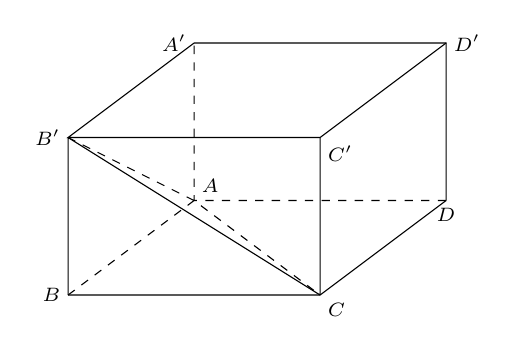
\begin{tikzpicture}[scale=0.8]
			\begin{scriptsize}
				\coordinate (A') at (0,2.5)    node at (A') [left] {$A'$};
				\coordinate (B') at (-2,1) node at (B') [left] {$B'$};
				\coordinate (C') at (2,1)  node at (C') [below right] {$C'$};
				\coordinate (D') at (4,2.5)    node at (D') [right] {$D'$};
				
				\coordinate (A) at (0,0)   node at (A) [above right] {$A$};
				\coordinate (B) at (-2,-1.5) node at (B) [left] {$B$};
				\coordinate (C) at (2,-1.5) node at (C) [below right] {$C$};
				\coordinate (D) at (4,0)   node at (D) [below] {$D$};
				
				\draw [dashed] (B)--(A)--(C) (D)--(A) (D)--(A)--(A') (A)-- (B'); 
				\draw (A')--(B')--(C')--(D');
				\draw (D)--(C)--(B);
				\draw (C)--(C') (B)--(B') (A')--(D')--(D) (B')--(C);
			\end{scriptsize}
		\end{tikzpicture}
	\end{center}
	\shortans{$2{,}36$}
	\loigiai{
	Chọn hệ trục tọa độ như hình vẽ.
	\begin{center}
		\begin{tikzpicture}[scale=0.8]
			\begin{scriptsize}
				\coordinate (A') at (0,2.5)    node at (A') [left] {$A'$};
				\coordinate (B') at (-2,1) node at (B') [left] {$B'$};
				\coordinate (C') at (2,1)  node at (C') [below right] {$C'$};
				\coordinate (D') at (4,2.5)    node at (D') [right] {$D'$};
				
				\coordinate (A) at (0,0)   node at (A) [above right] {$A$};
				\coordinate (B) at (-2,-1.5) node at (B) [left] {$B$};
				\coordinate (C) at (2,-1.5) node at (C) [below right] {$C$};
				\coordinate (D) at (4,0)   node at (D) [below] {$D$};
				
				\draw [dashed] (B)--(A)--(C) (D)--(A) (D)--(A)--(A') (A)-- (B'); 
				\draw (A')--(B')--(C')--(D');
				\draw (D)--(C)--(B);
				\draw (C)--(C') (B)--(B') (A')--(D')--(D) (B')--(C);
				\coordinate (x) at ($(B)+(-1.5,-1.1)$);
				%\coordinate (z) at ($(A')+(0,1)$);
				\coordinate (y) at ($(D)+(1,0)$);
				\draw [->] (B)--(x); 
				\draw [->] (A')--(z); 
				\draw [->] (D)--(y);
				\draw (x) node[below]{$x$};
				\draw (y) node[right]{$y$};
				\draw (z) node[left]{$z$};
			\end{scriptsize}
		\end{tikzpicture}
	\end{center}
	Ta có $A(0;0; 0)$, $C(4; 3; 0)$, $B'(4; 0; 5)$, $B(4; 0; 0)$.\\
	$G$ là trọng tâm của tam giác $ACB' \Rightarrow G\left(\dfrac{8}{3};1;\dfrac{5}{3}\right)$.\\
	$\overrightarrow{BG}=\left(-\dfrac{4}{3};1;\dfrac{5}{3}\right)\Rightarrow BG=\sqrt{\left(-\dfrac{4}{3}\right)^2+1^2+\left(\dfrac{5}{3}\right)^2}=\dfrac{5\sqrt{2}}{3}\approx 2{,}36.$
}
\end{ex}
%%%==============EX_12============%%%
\begin{ex}%[2H2V2-4]
	Cho tứ diện $ABCD$ có $AB, AC, AD$ đôi một vuông góc với nhau và $AD=2, AB=AC=1$. Gọi $I$ là trung điểm của đoạn thẳng $BC$ và $G$ là trọng tâm của tam giác $ABD$. Tính độ dài cạnh $IG$. (Kết quả làm tròn đến hàng phần trăm).
	\begin{center}
		\begin{tikzpicture}[scale=1, font=\footnotesize, line join=round, line cap=round]
			\foreach \x\y\t in {0/3/B,0/0/A,-1.2/-1.5/C,3/0/D}
			\coordinate (\t) at (\x,\y);
			\coordinate (I) at ($(B)!1/2!(C)$);
			\coordinate (M) at ($(B)!1/2!(D)$);
			\coordinate (G) at ($(A)!2/3!(M)$);
			\draw (B)--(C)--(D) (B)--(D);
			\draw[dashed] (B)--(A)--(C) (G)--(A)--(D) (A)--(I)--(G);
			\foreach \t/\g in {A/-90,B/180,C/-90,D/-90,I/180,G/-90}
			\draw[fill=white] (\t) circle(1.5pt)
			node[shift={(\g:9pt)}]{$\t$};
		\end{tikzpicture}			
	\end{center}
	\shortans{$0{,}85$}
	\loigiai{
		Vì tứ diện $ABCD$ có $AB, AC, AD$ đôi một vuông góc với nhau, nên ta chọn hệ trục tọa độ $Ax y z$ như hình vẽ (với $A$ là gốc tọa độ, đường thẳng $AC$ nằm trên trục $Ax, AD$ nằm trên trục $Ay$ và $AB$ nằm trên trục $Az$).
		\begin{center}
			\begin{tikzpicture}[scale=1, font=\footnotesize, line join=round, line cap=round]
				\foreach \x\y\t in {0/3/B,0/0/A,-1.2/-1.5/C,3/0/D}
				\coordinate (\t) at (\x,\y);
				\coordinate (I) at ($(B)!1/2!(C)$);
				\coordinate (M) at ($(B)!1/2!(D)$);
				\coordinate (G) at ($(A)!2/3!(M)$);
				\draw (B)--(C)--(D) (B)--(D);
				\draw[dashed] (B)--(A)--(C) (G)--(A)--(D) (A)--(I)--(G);
				\foreach \t/\g in {A/-90,B/180,C/-90,D/-90,I/180,G/-90}
				\draw[fill=white] (\t) circle(1.5pt)
				node[shift={(\g:9pt)}]{$\t$};
				\draw[->] (C) -- (-1.1,-1.5,2) node[anchor=north east]{$x$};
				\draw[->] (B) -- (0,4,0) node[anchor=north west]{$z$};
				\draw[->] (D) -- (4,0,0) node[anchor=south]{$y$};
			\end{tikzpicture}				
		\end{center}
		Khi đó $A(0;0;0)$, $B(0;0;1)$, $C(1;0;0)$ và $D(0;2;0)$.\\	
		Vì $I$ là trung điểm của $BC$ nên $I\left(\dfrac{1}{2};0;\dfrac{1}{2}\right)$.\\	
		$G$ là trọng tâm của tam giác $ABD\Rightarrow G\left(0;\dfrac{2}{3};\dfrac{1}{3}\right)$.\\
		Suy ra $\overrightarrow{IG}=\left(-\dfrac{1}{2};\dfrac{2}{3};-\dfrac{1}{6}\right)\Rightarrow IG=\sqrt{\left(-\dfrac{1}{2}\right)^2+\left(\dfrac{2}{3}\right)^2+\left(-\dfrac{1}{6}\right)^2}=\dfrac{\sqrt{26}}{6}\approx 0{,}85.$
	}
\end{ex}

\Closesolutionfile{ans}
